
\usetikzlibrary{graphs, positioning, quotes, shapes.geometric}
\chapter{预备知识}\label{chap:preliminary}{
	\section{侧信道攻击}
	密码硬件单元在运行过程中会产生多种不同物理形式的信息泄漏,如能量消耗、电磁辐射、执行时间、声音等。对于密码硬件单元的一次运行过程,攻击者可以对信息泄漏进行采样,获得信息泄漏的一个样本。攻击者可以令密码硬件单元多次运行,从而可以获得信息泄漏的多个样本,并把他们结合起来得到信息泄漏总体\footnote{客观存在的、在同一性质基础上结合起来的许多个别单位的整体。}$L$,它可以被描述为\equationref{eq:trace}的形式\footnote{本文使用数字或公式表述的次序从第0开始计数。有额外说明的情况除外。}。
	
	\begin{equation}
	L=L_{T\times M}
	=\begin{bmatrix}
		\Vector {l^{(0)}}\\
		\Vector {l^{(1)}}\\
		\vdots\\
		\Vector {l^{(T-1)}}
	\end{bmatrix}
	=\begin{bmatrix}
		l^{(0)}_0&l^{(0)}_1&l^{(0)}_2&\ldots&l^{(0)}_{M-1}\\
		l^{(1)}_0&l^{(1)}_1&l^{(1)}_2&\ldots&l^{(1)}_{M-1}\\
		l^{(2)}_0&l^{(2)}_1&l^{(2)}_2&\ldots&l^{(2)}_{M-1}\\
		\vdots&\vdots&\vdots&\ddots&\vdots\\
		l^{(T-1)}_0&l^{(T-1)}_1&l^{(T-1)}_2&\ldots&l^{(T-1)}_{M-1}\\
	\end{bmatrix}\label{eq:trace}
	\end{equation}
	
	\noindent 其中$l_i$($0\le i<T$)表示一个信息泄漏样本\footnote{本文中也将其称为一条迹(Trace)。},$T$表示信息泄漏样本量,$M$表示信息泄漏分量个数。如果攻击者获取的信息泄漏是能量消耗的形式,那么$L$也称为能量迹,$l_i$称为一条能量迹,$T$称为能量迹条数,$M$表示采集能量迹时设定的采样点个数;如果攻击者获取的信息泄漏是电磁场强度的形式,那么$L$也称为电磁迹,$l_i$称为一条电磁迹,$T$称为电磁迹条数,$M$表示采集电磁迹时设定的采样点个数,以此类推。密码硬件单元每次运行时,攻击者既对信息泄漏进行采样并记录,也对算法数据(明文和密文、签名消息的哈希值和消息签名等)的值、算法密钥的值进行记录。%我们把攻击者记录的算法数据、算法密钥总体记为$P,K$,其中$T$表示值的个数。
	
	使用$T$条迹和对应的算法数据恢复算法密钥的过程就是侧信道攻击。攻击者可能会使用额外的信息(算法实现的细节、被攻击的密码硬件单元的物理特性)或更适合的工具,使得信息泄漏模型对信息泄漏刻画更精确,从而更准确更高效地恢复算法的密钥。
	
	\subsection{信息泄漏模型}
	
	密码硬件单元在运行过程中会产生的信息泄漏可以用\equationref{eq:leakagemodel}表示。
	
	\begin{equation}
		\begin{cases}
			\Vector L=\begin{bmatrix}L_1&L_2&\cdots&L_{M-1}\end{bmatrix}:\mathcal \Omega\rightarrow \mathcal L=U^{M}\\
			P:\mathcal \Omega\rightarrow \mathcal P\\
			K:\mathcal \Omega\rightarrow \mathcal K
		\end{cases}\label{eq:leakagemodel}
	\end{equation}
	
	\noindent 其中,$\Omega$表示样本空间\footnote{一个随机试验中所有可能结果的集合。},$\mathcal L,\mathcal P,\mathcal K$分别表示信息泄漏$\Vector L$、算法数据$P$和算法密钥$K$的取值范围,$U$取决于采集信息泄漏的方式。\equationref{eq:leakagemodel}的含义是信息泄漏$\Vector L$是一个维度为$M$的随机变量,它的取值范围是$\mathcal L=U^M$,算法数据、算法密钥也是随机变量,它们的取值范围分别是$\mathcal P, \mathcal K$。
	
	\begin{example}
		如果一个密码硬件单元实现了AES-128加密算法,每次密码硬件单元加密16字节过程中使用示波器采集100个采样点的能量消耗,示波器使用8比特的位宽保存采样点,采样范围是-16V至16V,那么$U$=\{ -16, -15.875, -15.75, $\dots$, 15.75, 15.875\}是一个有256个元素的集合\footnote{集合中第$i$小的数$u_i$计算方式为$u_i=\frac{32}{2^8}(i-2^{8-1})$。},$\mathcal L=U^{100}$。$\mathcal K=\left( {\mathbb F_2^8}\right) ^{16}$,这表示AES-128算法的密钥是16个$\mathbb F_2^8$上的元素\footnote{AES-128加密算法在设置密钥、设置明文以及输出密文时以字节形式传输数据,但是内部的运算过程却在模多项式$x^8+x^4+x^3+x+1$的$\mathbb F_2^8$有限域上。这是因为一个字节的值可以和$\mathbb F_2^8$上的元素一一对应,例如字节值b'$\backslash$xcc'对应于$x^7+x^6+x^3+x^2$。本文使用字节以便用文字表述密钥、明文、密文的某些部分,使用$\mathbb F_2^8$以便用公式表述密钥、明文、密文相关概念。}。$\mathcal P=\left( {\mathbb F_2^8}\right) ^{16}\times \left( {\mathbb F_2^8}\right) ^{16}$,这表示AES-128算法的算法输入、输出各是16个$\mathbb F_2^8$上的元素。
	\end{example}
	
	\begin{example}
		如果一个密码硬件单元实现了ECDSA签名算法(具体参数见\ref{subs:ECDSAscheme}),Hash函数选为sha1\citep{FIPS180-4},每次密码硬件单元执行过程中使用示波器采集10000个采样点的能量消耗,示波器有无穷大的位宽保存采样点,那么$U=\mathbb R$是实数集,$\mathcal L=U^{10000}$。$\mathcal K=Z_q$,这表示签名私钥一定是模$q$整数环上的元素。$\mathcal P=\{0,1,\dots,2^{160}-1\}\times Z_q\times Z_q$,这表示消息的sha1杂凑值长度为160比特、签名算法输出的签名对$(r,s)$中$r,s$都是模$q$整数环上的元素。
	\end{example}
	
	
	本文使用小写字母表示对应的随机变量的样本值,即$\Vector l,p,k$分别表示$\Vector L,P,K$的样本值。如果出现需要表明这些样本值来自于哪一次采样结果的情况,我们使用带括号的数字上标对其进行区分。也就是说,采集到的迹$\Vector {l^{(0)}}, \Vector {l^{(1)}}, \dots, \Vector {l^{(T-1)}}$是信息泄漏$\Vector L$的$T$个样本值。攻击者记录到的多个算法密钥的值$k^{(0)}, k^{(1)}, \dots, k^{(T-1)}$是算法密钥$K$的$T$个样本值,攻击者记录到的多个算法数据的值$p^{(0)}, p^{(1)}, \dots, p^{(T-1)}$是算法数据$P$的$T$个样本值。
	
	密码设备的信息泄漏$\Vector L$依赖于设备正在处理的数据\footnote{这种数据的值称为中间值。},而敏感数据由算法数据和算法密钥计算得出。因此密码硬件单元的信息泄漏在某些时刻会受到算法密钥和算法输入的影响,如\equationref{eq:leakagedetail}所示。
	
	\begin{equation}
		\begin{cases}
			L_j=\omega_j h(y)+e_j,j\in\{0,1,2,\dots,M-1\}\\
			e_j\sim N(\mu_j,\sigma_j^2),j\in\{0,1,2,\dots,M-1\}\\
			y=g(p,k)
		\end{cases}\label{eq:leakagedetail}
	\end{equation}
	
	\noindent 其中,固定的常数$\omega$受密码设备本身和算法实现的影响,$e$为随机噪声,$\mu$为噪声本底值,$\sigma$为噪声标准差,$y$为敏感中间值,$p$为算法数据的值,$k$为算法密钥的值,$g$为敏感中间值的计算函数,它通常由被攻击的密码算法步骤选定,$h$为敏感中间值的信息泄漏转换函数,它通常由被攻击的密码设备类型决定,常用的转换函数有汉明重量函数$\mathrm {HW}(\cdot)$、汉明距离函数$\mathrm {HD}(\cdot,\cdot)$和最高有效位函数$\mathrm {MSB}(\cdot)$。敏感中间值$y$由函数$g$使用算法数据的值$p$和算法密钥的值$k$计算得出,因此它也可以看做一个随机变量的样本值,我们将这个随机变量记为$Y:\mathcal \Omega\rightarrow \mathcal Y$。随机变量$Y$的取值范围$\mathcal Y$取决于敏感中间值计算方式。
	
	\begin{example}\label{ex:aessw}
		在攻击AES-120加密算法软件实现主密钥第0字节时,通常选定$h(y)=\mathrm{HW}(y), y=g(p,k)=Sbox[p_0\oplus k_0]$,其中$p_0$表示明文第0字节(它是算法输入的一部分),$k_0$表示主密钥第0字节。$\mathcal Y=\mathbb F_2^8$。
	\end{example}

	\begin{example}
		在攻击AES-128加密算法硬件实现第10轮轮密钥第7字节时,通常选定$h(y)=\mathrm{HD}(y,c_7), y=g(p,k)=Sbox^{-1}[c_{11}\oplus k_{7}]$,其中$c_7,c_{11}$分别表示密文第7、11字节(它们是算法输出的一部分),$k_7$表示第10轮轮密钥第7字节。$\mathcal Y=\mathbb F_2^8$。
	\end{example}

	\begin{example}\label{ex:ecdsa}
		在攻击本文研究的双界面智能卡中ECDSA实现的数乘算法(见\algorithmref{alg:improvesignscalar})的第27次迭代时,会选定$h(y)=\mathrm{MSB}(y), y=g(p,k)=2\left( \left\lfloor \frac{s^{-1}(hsh+rd)\bmod q}{2^{256-27}}\right\rfloor \bmod 2\right)+\left( \left\lfloor \frac{s^{-1}(H(m_0)+rd)\bmod q}{2^{127-27}}\right\rfloor\bmod 2\right) $,其中$hsh$是算法输入,$r,s$是算法输出(他们都是算法数据),$q$是签名算法公开的固定参数,$d$是算法密钥。$\mathcal Y=\{1,2,3\}$。
	\end{example}
	\subsection{模板类侧信道攻击}
	
	侧信道攻击可以分为非模版类侧信道攻击和模板类侧信道攻击。在非模板类侧信道攻击中,差分能量攻击\citep{KocherJJ99, Messerges00, BevanK02}和相关能量攻击\citep{Brier04}是最基本也是最常用的攻击方法。差分能量攻击对密钥$k$的值进行猜测,使用敏感中间值$y$划分能量迹,计算能量迹之间的差异来确定密钥;相关能量分析对密钥$k$的值进行猜测,结合信息泄漏转换函数$h$和敏感中间值$y$估计理论上的能量消耗,计算能量迹与估计的能量消耗之间的相关系数来确定密钥。
	
	模板类侧信道攻击使用模版对常数$\omega$、信息泄漏转换函数$h$以及噪声$e$进行描述,使得对信息泄漏的刻画比非模板类侧信道攻击更精确。模板类侧信道攻击的优势在于,它有可能仅使用信息泄漏的一个样本并结合算法输入的值恢复算法密钥的值。模板类侧信道攻击分为建模和攻击两个阶段,建模阶段对迹的特征进行刻画,第二个阶段利用该特征进行攻击\citep{Mangard07}。
	
	模板类侧信道攻击分为两个阶段,为了区分两个阶段使用的数据,我们使用下标$t,a$进行区分。在建模阶段,攻击者可以根据$T_t$条迹以及对应的算法密钥、算法数据进行建模;在攻击阶段,攻击者采集$T_a$条迹和对应的算法数据,使用全部或者其中的一部分恢复算法密钥。
	
	在建模阶段,攻击者可以对迹的特征进行刻画,这意味着攻击者可以确定出某个或某些操作的模版。例如,攻击者可以拥有一台与被攻击设备类型相同的设备,并且该设备完全由攻击者控制。攻击者可以让设备多次运行,每次运行前设定不同的算法输入、算法密钥,记录对应的迹(如能量迹、电磁迹)和算法输出。对特定敏感中间值构建模版是常见的构建策略,攻击者可以在不对敏感中间值的信息泄漏转换函数$h$做任何假设的情况下,根据算法数据的值$p$和算法密钥的值$k$计算敏感中间值$y$,把对应相同中间值的迹分为一组,并对每一组构造模版。
	
	在攻击阶段,攻击者可以利用特征从被攻击设备获得的迹来确定密钥。对于一条迹$\Vector l\in \Vector L_{T_a\times M}$,攻击者可以检查迹和每一个中间值$y\in\mathcal Y$所对应模版的匹配程度$d_1(y)$(下标1表示仅使用一条迹计算匹配程度),这种匹配程度可以量化,其具体计算方法取决于构造模板的工具。依据极大似然原理,正确模版理论上应该与最高的匹配程度相对应\citep{Kay1998}。攻击者选取最高匹配程度所对应的敏感中间值作为实际敏感中间值的估计$\hat y$,即$\hat y=\mathop{\mathrm{argmax}}\limits_{y\in\mathcal Y}\left\lbrace d_1(y)\right\rbrace $。
	
	在算法数据给定的情况下,算法密钥和敏感中间值有对应关系。如果在算法输入不变的情况下,对于不同的算法(子)密钥的值,函数$g$计算出的敏感中间值一定不同\footnote{单射。},那么迹和中间值$y$所对应的模版的匹配程度$d_1$和(子)密钥的值关联起来,如\equationref{eq:gsup-1}所示,本文将$\tilde d_1(k)$称为密钥值$k$的得分。在此基础上,攻击者得到算法(子)密钥的值的估计,如\equationref{eq:1tracek}所示。
	
	\begin{equation}\label{eq:gsup-1}
		\tilde d_1(k)=d_1\left(g(p,k) \right)=d_1(y)
	\end{equation}
	
	\begin{equation}\label{eq:1tracek}
		\hat k=\mathop{\mathrm{argmax}}\limits_{k\in\mathcal K}\left\lbrace \tilde d_1(k)\right\rbrace 
	\end{equation}
	
	如果函数$g$有可能在算法输入不变的情况下将不同(子)密钥映射到同一个中间值,那么无法直接对算法(子)密钥的值进行估计。尽管如此,这种情况下攻击者也能了解到关于算法密钥的信息,减小枚举空间。
	
	\begin{example}
		在\exampleref{ex:aessw}中,$\hat k_0=\mathop{\mathrm{argmax}}\limits_{k_0\in\mathbb F_2^8}\left\lbrace d_1\left(Sbox\left[p_0\oplus k_0\right]\right)\right\rbrace $,其中$k_0$表示主密钥第0字节的取值。
	\end{example}

	\begin{example}
		在\exampleref{ex:ecdsa}中,找不到合理的子密钥划分使得函数$g$有单射性质,尽管知道了关于算法密钥$d$的信息但是还是不能恢复它任何一个比特的数值。结合数学方法,我们可以利用多处关于算法密钥的信息来恢复完整的算法密钥,见\ref{subs:infoforlattice}。
	\end{example}
	
	如果被攻击设备的算法密钥没有使用次数限制或次数限制足够大,那么攻击者可以从令被攻击设备运行$T_a$次\footnote{具体次数受算法密钥次数、攻击者所能接受的攻击时间共同决定。例如,对于AES-128加密算法无防护软件实现,有可能仅使用一条能量迹就恢复算法密钥,那么此时令$T_a=1$已经足够完成攻击。对于本文研究的双界面智能卡ECDSA实现,理想情况下采集十万条能量迹有助于减少利用信息泄漏恢复实际私钥的时间,但是受采集时间限制只能令$T_a=5000$。}并获取多条迹和对应的算法数据的值,在这之后选取一些能量迹进行攻击并综合估计(子)密钥的值$\hat k$,如\equationref{eq:ttracek}所示。
	
	\begin{equation}\label{eq:ttracek}
		\begin{cases}
			\hat k=\mathop{\mathrm{argmax}}\limits_{k\in\mathcal K}\left\lbrace \tilde d_t(k)\right\rbrace \\
			\tilde d_t(k)=\sum\limits_{i\in \mathcal I}\tilde d^{(i)}_1(k)\\
			\mathcal I\subset \{0,1,2,\dots,T_a-1\}\\
			t=\vert\mathcal I\vert
		\end{cases}
	\end{equation}
	
	\noindent 其中,元素个数为$t$的集合$\mathcal I$描述了攻击者从采集到的$T_a$条迹中选取哪些迹用于实际攻击。
	
	\begin{example}
		在\exampleref{ex:aessw}中,假设攻击者采集了100条能量迹,那么他可以组合不超过100条能量迹所提供的信息。进一步假设攻击者组合后50条能量迹的信息。对于第$i$条($50\le i<100$)能量迹能量迹$\Vector {l^{(i)}}$,攻击者可以计算迹和特定中间值所对应模版的匹配程度,并据此算出匹配程度和主密钥第0字节的值的对应关系。接着他组合这些信息推断子密钥$\hat k_0=\mathop{\mathrm{argmax}}\limits_{k_0\in\mathbb F_2^8}\left\lbrace \sum\limits_{i=50}^{99}d_1^{(i)}\left( Sbox[p^{(i)}_0\oplus k_0]\right)\right\rbrace $。
	\end{example}
	%假如攻击者希望综合前$t$($t\le T_a$)条迹的信息,他能每一条迹$\Vector{l_i},0\le i<t$和对每种中间值猜测都能计算其得分$d_1^{(i)}(y)$。假如$g_p^{-1}$存在,攻击者可以这么估计密钥$\hat k$
	
	按照构造模板的工具对模板类侧信道攻击进行划分,可以大致分为传统模板攻击和基于深度学习的侧信道攻击。
	\subsubsection{传统模板攻击}
	
	在传统模板攻击中,使用多元正态分布构造模版、刻画迹的特征。模板类侧信道攻击中量化迹和每一个模版的匹配程度的方法是计算条件概率的对数值。
	
	构建一个中间值$y$所对应的模版,就是使用所有中间值都是$y$的迹对均值向量和协方差矩阵$\Vector {\mu_y},\Sigma_y$进行估计。这两个参数的含义是,在中间值为$y$的条件下,信息泄漏$\Vector L$应当服从均值为$\Vector {\mu_y}$协方差为$\Sigma_y$的多元正态分布,其条件概率密度函数如\equationref{eq:f(b|a)}所示。
	
	\begin{equation}\label{eq:f(b|a)}
		f\left(\Vector L=\Vector l|Y=y \right)=\frac{e^{\frac{-1}2(\Vector l-\Vector {\mu_y})\Sigma_y^{-1}(\Vector l-\Vector {\mu_y})}}{\sqrt{(2\pi)^M\det (\Sigma_y)}}
	\end{equation}
	
	%构建一个中间值$y$所对应的模版,就是根据所有中间值都是$y$的迹,计算出此时信息泄漏应当服从的多元正态分布的条件概率分布$f\left(\Vector L|Y=y \right) $。多元正态分布的概率密度函数由均值向量和协方差矩阵完全确定,因此只用使用所有中间值都是$y$的迹对均值向量和协方差矩阵$\vector {\mu_h},\Sigma_h$进行估计即可。
	
	量化迹和每一个模版的匹配程度的方法是根据贝叶斯公式计算条件概率,如\equationref{eq:pr(a|b)}所示,其中$\mathrm{Pr}\left[Y=y \right]$的数值容易用理论推算,$f\left(\Vector L=\Vector l\right)$的数值容易从建模的迹中推算。
	
	\begin{equation}\label{eq:pr(a|b)}
		\mathrm{Pr}\left[Y=y|\Vector L=\Vector l \right]=\frac{f\left(\Vector L=\Vector l|Y=y \right)\mathrm{Pr}\left[Y=y \right]}{f\left(\Vector L=\Vector l\right)}
	\end{equation}
	
	量化迹和每一个模版的匹配程度使用公式$d_1(y)=\log \mathrm{Pr}\left[Y=y|\Vector L=\Vector l \right]$。
	\subsubsection{基于深度学习的侧信道攻击}
	在基于深度学习的侧信道攻击中,使用深度神经网络构造模版、刻画迹的特征。模板类侧信道攻击中量化迹和每一个模版的匹配程度的方法是使用模型的预测结果。
	
	使用深度神经网络构造模版,首先要构造训练集。训练集由两部分构成,训练数据是信息泄漏样本总体$L_{T_t\times M}$,训练标签是敏感中间值总体$y^{(0)},y^{(1)},\dots,y^{(T_t-1)}$。将训练集输入深度神经网络后就得到了训练好的模型。
	
	模型可以对输入的迹$\Vector l$进行预测,输出一个概率向量$\Vector \pi$。向量的分量$\pi_y$表示模型预测迹$\Vector l$对应于中间值$y$的概率。量化迹和每一个模版的匹配程度使用公式$d_1(y)=\log \pi_y$。
	\subsection{侧信道评估指标}
	\subsubsection{测试向量泄漏评估}
	比攻击算法实现略微简单一点的需求是检测算法实现是否存在信息泄漏。在侧信道分析中,测试向量泄漏评估\citep{Goodwill2011,Becker2013,ISO/IEC17825}(Test Vector Leakage Assessment,TVLA)是对采集到的电磁迹中每一个采样点进行单变量检测以判断该组电磁迹是否存在信息泄漏的检测框架。对于第$j$个采样点,泄漏检测的零假设为“$\mathrm H_0:$第$j$个采样点不存在信息泄漏”,备择假设为“$\mathrm H_1:$第$j$个采样点存在信息泄漏”。如果原假设$\mathrm H_0$成立,那么第$j$个采样点的电磁场幅度应该是某种随机噪声的样本值,因此可以这么表述原假设和备择假设:
	
	$$\begin{cases}\mathrm H_0:\exists \mu_j,\exists\sigma_j,\exists  {L_j}\sim N(\mu_j,\sigma_j^2),\forall 0\le i<T,l_{i,j}\mbox{是} {L_j}\mbox{样本值}\\\mathrm H_1:\forall \mu_j,\forall\sigma_j,\not\exists  {L_j}\sim N(\mu_j,\sigma_j^2),\forall 0\le i<T,l_{i,j}\mbox{是} {L_j}\mbox{样本值}\end{cases}$$
	
	当单变量检测的统计量被观测到的概率低于显著性水平$\alpha$时\footnote{显著性水平$\alpha$可以任意选择。在侧信道分析中,显著性水平通常设置为$10^{-5}$。},我们拒绝原假设$\mathrm H_0$,接受备择假设$\mathrm H_1$,即有超过$(1-\alpha)$的把握认为第$j$个采样点存在信息泄漏。
	
	本文在TVLA框架下使用的单变量检测是Welch's T检验\citep{Welch38}。使用某种方法\footnote{对于本文评估ECDSA实现电磁迹的信息泄漏,依据电磁迹所对应的$t_i$的值进行划分。}划分所有电磁迹第$j$个采样点构成的总体$\{l_{0,j},l_{1,j},\dots l_{T-1,j}\}$得到两个互不相交的总体,记为$L_{A,j},L_{B,j}$。我们将这两个总体的样本数量分别记为$n_A,n_B$,将其样本均值分别记为$\overline{x_{A,j}},\overline{x_{B,j}}$,将其样本标准差分别记为$s_{A,j},s_{B,j}$。在之后,使用统计量$v_j$来描述它们的差异。统计量$v_j$的计算方式如\equationref{eq:calct}所示。
	
	\begin{equation}\label{eq:calct}
		v_j=\frac{\overline {x_{A,j}}-\overline{x_{B,j}}}{\sqrt{\frac{s_{A,j}^2}{n_A}+\frac{s_{B,j}^2}{n_B}}}
	\end{equation}
	
	如果原假设$\mathrm H_0$成立,那么统计量$v_j$应当服从自由度为$f_j$的T分布,即$v_j\sim t(f_j)$,其中$f_j$计算方法如\equationref{eq:calcdegoff}所示。
	
	\begin{equation}\label{eq:calcdegoff}
		f_j=\frac{\left(\frac{s_{A,j}^2}{n_A} +\frac{s_{B,j}^2}{n_B}\right)^2 }{\frac{s_{A,j}^4}{n_A^2(n_A-1)}+\frac{s_{B,j}^4}{n_B^2(n_B-1)}}
	\end{equation}
	
	此时可以计算统计量$v_j$所对应的p值,其计算方式如\equationref{eq:calcp}所示。
	
	\begin{equation}\label{eq:calcp}
		p_j=2\left( 1-F_T(\vert v_j\vert ,f_j)\right) 
	\end{equation}
	
	\noindent 其中,$F_T(\cdot,f_j)$表示自由度为$f_j$的T分布的累积分布函数,当自由度较大($f_j>50$)时,T分布的累积分布函数可以用标准正态分布的累积分布函数$\Phi(\cdot)$加以近似。
	
	统计量阈值$th_j$与显著性水平$\alpha$有对应关系,因此可以通过T分布的累积分布函数计算得到$th_j=F_T^{-1}\left( 1-\frac\alpha2,f_j\right) $。在侧信道分析中,通常选取$\alpha=10^{-5}$,当样本总量足够大(超过50),自由度一般较大($f_j>50$),用$\Phi(\cdot)$近似$F_T(\cdot,f_j)$时可以算出$th_j=4.417\approx4.5$。
	
	\subsubsection{猜测熵}
	猜测熵(Guessing Entropy,GE)由Standaert等\citep{Standaert09}提出。正确密钥猜测熵是针对分组密码算法的侧信道攻击中使用广泛的度量评估指标,它能够反映将侧信道攻击与穷举密钥结合使用时进行攻击的复杂度。
	
	猜测熵是一种依赖于攻击方法的评估指标。攻击者需要使用某种方法,选定攻击所使用的能量迹条数$t$,对分组密码算法的一个(子)密钥进行多次互相独立的攻击,记录每次攻击中某个(子)密钥值$k$得分$d_t(k)$在所有密钥得分中的排名$r_t(k)$,最后取排名的均值$\mathbb E\left(r_t(k) \right) $作为该密钥值$k$的猜测熵$GE_{t}(k)$。排名的计算方式是$r_t(k)=\left\vert\left\lbrace j\in\mathcal K|d_t(j)>d_t(k)\right\rbrace  \right\vert $,其中$\vert\cdot\vert$表示集合中元素的个数。
	
	\begin{example}\label{ex:badge}
		在\exampleref{ex:aessw}中,主密钥第0字节的值被设置为204。攻击者使用传统模板攻击作为攻击方法,每次随机选择100条能量迹进行攻击,攻击5次。5次攻击所计算出的密钥得分如下表所示。
		
		\begin{table*}[!h]
			\caption{密钥得分示例}
			\scriptsize{
				\begin{tabular}{cc|cccccccccccccc}
					\hline
					\multicolumn{2}{c|}{\multirow{2}{*}{密钥得分}} & \multicolumn{14}{c}{密钥值} \\
					%\cline{3-5}
					\multicolumn{2}{c|}{}
					    &     0 & \dots &    76 & \dots &   140 & \dots &   200 & \dots &   204 &   205 & \dots &   236 & \dots &   255\\
					\hline
					\multirow{5}{*}{攻击编号} 
					& 1 & 0.073 & \dots & 0.878 & \dots & 0.984$^*$ & \dots & 0.575 & \dots & 0.910 & 0.590 & \dots & 0.957$^*$ & \dots & 0.161\\
					
					& 2 & 0.208 & \dots & 0.861 & \dots & 0.659 & \dots & 0.609 & \dots & 0.939 & 0.904 & \dots & 0.722 & \dots & 0.240\\
					
					& 3 & 0.095 & \dots & 0.518 & \dots & 0.762$^*$ & \dots & 0.963$^*$ & \dots & 0.690 & 0.568 & \dots & 0.702$^*$ & \dots & 0.313\\
					
					& 4 & 0.228 & \dots & 0.962$^*$ & \dots & 0.674 & \dots & 0.733 & \dots & 0.884 & 0.643 & \dots & 0.617 & \dots & 0.253\\
					
					& 5 & 0.131 & \dots & 0.684 & \dots & 0.975$^*$ & \dots & 0.776 & \dots & 0.808 & 0.942$^*$ & \dots & 0.933$^*$ & \dots & 0.064\\
					
					\hline
				\end{tabular}
			}
			\tabnote{在某一次攻击中,如果错误密钥的得分超过正确密钥的得分,那么错误密钥的得分右上角使用星号*标记。}
		\end{table*}
	
		为了方便解读,不妨假设未列举出来的其他密钥值的得分都小于0.5。观察表格容易知道,在5次攻击中,密钥值204的得分在所有得分的排名中分别位于第三位\footnote{本文使用汉字表述的次序从第一开始计数,有额外说明的情况除外。}、第一位、第四位、第二位、第四位。因此在每次使用100条能量迹进行传统模板攻击时,密钥值204的猜测熵为$GE_{100}(204)=\frac15$(2+ 0+ 3+ 1+ 3)= 1.8。同理可以算出其他每种密钥值的猜测熵,如密钥值140的猜测熵为$GE_{100}(140)=\frac15$(0+ 4+ 1+ 3+ 0)= 1.6,密钥值205的猜测熵为$GE_{100}(205)=\frac15$(4+ 1+ 4+ 4+ 1)= 2.8。因为正确密钥是204,所以正确密钥猜测熵是1.8。
	\end{example}
	\subsubsection{成功条数}
	成功条数\citep{Kim14}(Measurements To Disclosure,MTD)定义为攻击成功时所使用的迹的最少条数,它能反映侧信道攻击在
	攻击阶段的时间消耗\footnote{采集迹、使用迹进行攻击的时间都和迹的条数成正比。}。成功条数计算方式为$T^*=\min\limits_{0<t\le T_a}\left\lbrace t:GE_t(k^*)=0 \right\rbrace $,其中$k^*$表示正确的(子)密钥。如果攻击不成功,那么成功条数无意义。在\exampleref{ex:badge}中,根据已有数据只能推算出$T^*\le100$。
	\subsubsection{成功率}
	成功率定义为多次攻击互相独立的情况下,成功恢复(子)密钥的次数与攻击次数的比值。在\exampleref{ex:badge}中,成功率为0.2。它直观地反映侧信道攻击在多大程度上能恢复密钥。成功率和攻击时间通常是负相关的,但它不能直接反映攻击时间。
	%猜测熵、成功率、猜测熵收敛速度(研究内容1)、真阳性率(研究内容2)
	\section{数据增强}
	
	\subsection{侧信道攻击领域数据增强}
	数据增强方法可以提高DL-SCA的攻击效果。
	
	Cagli等\citep{Cagli17}在2017年提出了一种数据增强方法,通过使用位移变形(见\algorithmref{alg:SH})和添加删除变形(见\algorithmref{alg:AR}),分别模拟随机延迟和时钟抖动的技术效果进而合成新的迹,以提升原始DL-SCA技术效果。位移变形有两个可变的参数$lb,rb$\footnote{因为深度神经网络输入尺寸是个定值且深度神经网络不接受输入尺寸以外的数据,因此$M^\prime$必须恰好等于深度神经网络输入尺寸,$M^\prime$不是可变参数。},它们分别描述了可能被截取的迹的起始采样点的下界和上界。添加删除变形有一个可变的参数$R$,它描述了时钟抖动的剧烈程度。对于Cagli等的数据增强方法实现,调用一次数据增强实现只能合成一条新的迹,为了构造训练集需要调用多次数据增强实现。
	
	Pu等\citep{Pu17}采用循环位移变形(见\algorithmref{alg:RO})的方法来实现数据增强,大致思想与Cagli等\citep{Cagli17}的位移变形类似,但是它避免了数据增强后一条迹的采样点个数减小的问题。循环位移变形有两个可变参数$\gamma,C$,它们分别描述了实际循环位移幅度与采样点个数比值的上界、一条能量迹所合成的新的迹的数量。对于Pu的数据增强方法实现,调用一次数据增强实现可以合成多条新的迹,这使得构造训练集只需要调用一次数据增强实现。
	
	Kim等\citep{Kim19}提出向神经网络批归一化\footnote{在每个批次上独立地归一化。}处理后的数据添加高斯白噪声(见\equationref{eq:addnoise})可以解决过拟合问题,从而显著提升池化模板攻击的攻击效果。在添加高斯白噪声的方法中,可变的参数是$\alpha$,它描述了噪声的方差。实际操作中可以在深度神经网络训练之前向训练数据叠加噪声矩阵,实现和\equationref{eq:addnoise}等效的效果,但是这需要额外增加参数来修正噪声方差并调整归一化函数。
	
	\begin{equation}\label{eq:addnoise}
		 {L_{batch}^{agmt}}=BN_0(L_{batch})+\Psi,\Psi\sim N(0,\alpha)
	\end{equation}
	
	\noindent 其中,$L_{batch}$表示训练数据$L$分批后的张量\footnote{在深度神经网络训练之前,训练数据会执行分批操作,它会由二维(两个维度分别表示迹的条数、一条迹的采样点个数)矩阵变成了三维(三个维度分别表示批次数、一个批次的迹的条数、一条迹采样点个数)的张量。分批操作的输入和输出有对应关系,他们是相同数据的不同表现形式。},$BN_0$表示批归一化函数,$\Psi$表示一个每个元素互相独立且都服从正态分布的噪声张量。
	
	Picek等\citep{Picek19}于2019年首次提出用SMOTE(见\algorithmref{alg:smotepolulate})解决样本不平衡的问题,这使得使用敏感中间值的汉明重量作为训练标签时,基于深度学习的侧信道攻击的技术效果有所提升。SMOTE的核心是:特征空间上邻近的点其特征都是相似的。SMOTE并不是在数据空间上进行采样,而是在特征空间中进行采样,所以它的准确率会高于传统的采样方式。SMOTE有两个可变的参数$n,C$,它们分别描述了寻找最近的迹的数目以及一条迹所需要合成的新的迹的数目。对于SMOTE实现,调用一次数据增强实现可以合成多条新的迹,这使得构造训练集只需要调用一次数据增强实现。
	
%	Won等\citep{Won20}在Picek等\citep{Picek19}工作基础上,系统地研究了SMOTE及其多种变体\citep{Kovcs19}实现数据增强的技术效果,并发现SMOTE、CURE\_SMOTE、ASMOBD、MCT和MOT2LD相对来说有优良的技术效果。
%	Luo等\citep{Luo21}首次提出在基于深度学习的侧信道攻击中利用混淆(Mixup)技术实现数据增强,以扩大训练集,提供攻击成功率。该方法的核心思想是每次随机选取两条迹,并以一定的比例插值生成新的迹。与此同时,训练标签也需要重新生成,新的训练标签应当是迹所对应标签的one-hot编码进行同样比例插值的结果。训练过程只采用插值合成的新的训练数据和训练标签,不使用混淆前的训练数据和训练标签。
%	
%	Mukhtar等\citep{Mukhtar22}于2022年提出了一种基于条件生成对抗网络和连体网络的数据增强方法,从而提高了攻击能力。在分组和公钥密码算法实现的泄漏数据集上的定量分析显示,此方法可以生成逼真的含有信息泄漏的迹,使用数据增强后的迹用于训练可以完成攻击(而不进行数据增强就不能完成攻击)。
	\subsection{图像识别领域数据增强}
	
	在图像识别领域,也有相关工作给本文研究内容带来启发。
	
	\begin{figure}[!h]
		\begin{center}
			\begin{tikzpicture}[node distance=25pt]
			\node[draw, rounded corners,align=center] at(4,1.5) (step2)  {数据增强策略S};
			\node[draw, rounded corners,align=center] at(2,3) (step1)  {控制器(RNN)};
			\node[draw, rounded corners,align=center] at(2,0) (step3)  {子网络};
			\node[draw, rounded corners,align=center] at(0,1.5) (step4)  {验证准确率R};
			
			\draw[->] (step1) -| (step2);
			\draw[->] (step2) |- (step3);
			\draw[->] (step3) -| (step4);
			\draw[->] (step4) |- (step1);
			\end{tikzpicture}
			\bicaption{\enspace 应用Autoaugment的框架总览}{\enspace Overview of Autoaugment Framework}
			\label{fig:autoaugment}
		\end{center}
	\end{figure}
	
	Autoaugment\citep{Cubuk19}是一个简单的程序,它将寻找最优数据增强策略问题表述为离散搜索问题,如\figureref{fig:autoaugment}所示,它能自动地改进图像分类的数据增强策略。从图中可以看出一次循环分入如下步骤:搜索算法对数据增强策略S进行采样、使用数据增强策略S训练子网络、子网络对验证集进行预测、反馈验证准确率R以调整控制器。该程序的核心是:数据增强策略S会被用于训练神经网络,神经网络的验证准确率会反过来对控制器进行更新。程序可变的部分是控制器、数据增强策略搜索空间、子网络。搜索出最佳数据增强策略后,多次对原始图像执行数据增强策略即可获得训练集。
	
	
	\section{模拟退火}
	模拟退火算法(Simulated Annealing)是一种基于模拟物质退火过程的启发式优化算法。它模拟了固体物质在高温下退火冷却过程中的行为,通过随机搜索和概率性接受劣解的策略,寻找全局最优解或接近最优解的近似解。
	
	模拟退火算法最初由Metropolis等\citep{Metropolis53}于1953年受到固体物理学中的退火原理的启发提出,并在1983年由Kirkpatrick等\citep{Kirkpatrick83}引入到组合优化领域。在该算法中,优化问题被视为能量最小化的问题,其目标是通过降低系统能量来寻找最优解。
	
	算法的基本思想是,从一个初始解开始,通过一系列的状态转移来搜索解空间。在搜索过程中,模拟退火算法会接受一定概率上的劣解,以避免陷入局部最优解。随着搜索的进行,算法会逐渐降低温度(控制接受劣解的概率),使得在初始阶段更容易接受劣解,而在后续阶段更倾向于接受更好的解\citep{Steinbrunn1997}。这种温度的降低过程类似于物质退火过程中的冷却。
	
	模拟退火算法的关键在于状态转移的策略。一般来说,它包括生成邻域解、计算能量差和接受概率等步骤。邻域解的生成可以通过扰动当前解来实现,能量差用于衡量解的质量,接受概率则基于能量差和当前温度计算得出。通过不断迭代搜索和状态转移,模拟退火算法可以在解空间中进行全局搜索,并最终找到一个较优的解。算法伪代码如\algorithmref{alg:sa}所示。
	
	\begin{algorithm}[!h]
		\caption{模拟退火算法}\label{alg:sa}
		\begin{algorithmic}[1]
			\Statex \textbf{输入:} $state$:随机初始解
			\Statex \textbf{输入:} $inittemp$:初始温度
			\Statex \textbf{输入:} $\gamma\in(0,1)$:退火速度
			\Statex \textbf{输入:} $n$:迭代次数
			\Statex \textbf{输入:} $Energy(\cdot)$能量函数,用于计算解对应的能量值
			\Statex \textbf{输出:} $minstate$:(近似)最优解
			\State $cost := Energy(state),mincost:=cost,minstate:=state,temp\gets inittemp$
			\For{$i = 0, \dots, n-1$}
				\Repeat
					\State 对$state$进行扰动得到$newstate$\Comment{扰动当前解,生成邻域解}
					\State $newcost:=Energy(newstate)$
					\If {$cost-newcost\ge0$}\Comment{计算能量差}
						\State $state:= newstate$
						\State $cost:= newcost$
					\Else
						\State $p\gets U(0,1)$
						\If{$p\le e^{-\frac{cost-newcost}{temp}}$}\Comment{计算能量差和接受概率}
							\State $state:= newstate$
							\State$cost:= newcost$
						\EndIf
					\EndIf
					\If {$mincost\ge cost$}
						\State $minstate:= state$\Comment{记录优于最优解的当前解}
						\State $mincost:= cost$
					\EndIf
				\Until {达到平衡}
				\State $temp\gets temp\times\gamma,i\gets i+1$\Comment{降低温度}
			\EndFor
			\State \Return $minstate$
		\end{algorithmic}
	\end{algorithm}

	\section{椭圆曲线数字签名算法}
	椭圆曲线数字签名算法(Elliptic Curve Digital Signature Algorithm,ECDSA)是一种基于椭圆曲线密码学的数字签名算法。它被广泛应用于信息安全领域,用于验证数据的完整性和身份认证。
	
	ECDSA基于椭圆曲线上的离散对数困难问题,利用椭圆曲线上的点运算来实现安全的加密和签名机制,具有较高的安全性和较小的计算复杂度。椭圆曲线上的点的数乘(Scalar Multiplication)实现方式是基于椭圆曲线上的群运算特性,通过重复应用点加法(Add)和点倍乘(Double)操作,实现椭圆曲线上的点的数乘。椭圆曲线上的点的数乘结果依然是椭圆曲线上的点,即$\forall 0\le i\le q,\forall P\in E, i\cdot P\in E$。
	
	\subsection{一种ECDSA实际方案}\label{subs:ECDSAscheme}
	接下来以SP 800-186\citep{SP800-186}指定的Weierstrass曲线NIST P-256为例,介绍ECDSA的基础原理的相关知识。
	
	\textbf{密钥生成}:NIST P-256规定了椭圆曲线$E$和生成元$G\in E$。$q$为曲线$E$的加法阶。
	
	
	\begin{equation}\label{eq:P256}
	\small
	\begin{cases}E:y^2=x^3+ax+b \pmod {P_E}\\
	G=(g_x,g_y)\\
	a=-3\\
	b=\mathtt{0x5ac635d8aa3a93e7b3ebbd55769886bc651d06b0cc53b0f63bce3c3e27d2604b}\\
	P_E=2 ^ {256} − 2 ^ {224} + 2 ^ {192} + 2 ^ {96} − 1\\
	g_x=\mathtt{0x6b17d1f2e12c4247f8bce6e563a440f277037d812deb33a0f4a13945d898c296}\\
	g_y=\mathtt{0x4fe342e2fe1a7f9b8ee7eb4a7c0f9e162bce33576b315ececbb6406837bf51f5}\\
	q=\mathtt{0xffffffff00000000ffffffffffffffffbce6faada7179e84f3b9cac2fc632551}
	\end{cases}
	\end{equation}
	
	签名者选取一个256bit随机数$\sk$作为私钥并计算$\pk=\sk\cdot G$。$\sk$和$\pk$分别是签名者的私钥和公钥,$\sk$保密,$\pk$公开。
	
	\textbf{签名过程}:对于消息$m_0$,签名者每次秘密选取256bit整数$1<\nonce<q$\footnote{一次性随机数(Number once,Nonce),它是一个只被使用一次的随机数值。},计算这些值:
	
	\begin{equation}\label{eq:sign}
		\begin{cases}
			Q=\nonce\cdot G\\
			r=Q.x\bmod q\\
			hsh=H(m_0)\\
			s=\nonce^{-1}(hsh+r\cdot\sk) \bmod q
		\end{cases}
	\end{equation}
	
	上述签名过程\footnote{在某些文献中,签名中$s$的计算方式是$s=k^{-1}(hsh+r\cdot x)\bmod q$,这是因为它们表示私钥和一次性随机数的变量名和本文不同。}中,$Q.x$表示取椭圆曲线上的点$Q$的横坐标,$H$是一个安全的Hash函数,$m_0$是要签名的消息,$\nonce$是随机秘密选取的整数。数值对$(r,s)$记为消息的签名。
	
	如果随机数$\nonce$存在泄漏,那么攻击者有可能依据公开的参数$E,G$、公钥$P$、哈希函数$H$、签名消息$m_0$、签名$(r,s)$和随机数$\nonce$的信息泄漏,构造与私钥$\sk$和有关的方程并使用数学方法恢复私钥$\sk$,实现伪造签名、篡改数据和身份欺骗。
	
	\textbf{验签过程}:对于消息$m_0$,验证者可以计算
	\begin{equation}\label{eq:prepare-verify}
	\begin{cases}
		u_1=s^{-1}r\bmod q\\
		u_2=s^{-1}H(m_0)\bmod q\\
		R=u_1\cdot \pk+u_2\cdot G
	\end{cases}
	\end{equation}
	
	如果$R.x=r$,那么验证者可以确认$(r,s)$是签名者对消息$m_0$的有效签名;否则,签名无效。数字签名可以实现对消息的认证,推导过程如\propositionref{prop:ECDSA-authentication}所示。
	
	\subsection{一种ECDSA中的数乘实现}
	Roche等\citep{Roche21}对使用了SmartMX\citep{p5x}安全微控制器芯片中ECDSA中的数乘实现进行了研究并进行合理的猜想,最终通过数乘实现中敏感随机数的泄漏恢复了使用SmartMX\citep{p5x}的\textit{Google Titan Security Key}\citep{Titan}的私钥。
	
	ECDSA的签名操作和验签操作会不可避免地对椭圆曲线上的点进行数乘,如\equationref{eq:sign}中$\nonce\cdot G$、\equationref{eq:prepare-verify}中$u_1\cdot \pk$和$u_2\cdot G$所示。Roche等\citep{Roche21}首先分析了验签操作中的数乘实现的电磁迹,根据预计算时间非常长、乘数是256比特、迭代次数是128、每次点加法之前只有一次点倍乘操作、有的迭代中缺少点加法操作等信息,综合推断验签操作中的数乘算法使用了梳子\citep{Lim94}实现。
	
	Roche等\citep{Roche21}对梳子方法进行了猜测\footnote{对于第一次数乘,$\multiplier=u_1,P=\pk$;对于第二次数乘,$\multiplier=u_2,P=G$。}:
	
	\begin{itemize}
		\item 使用\algorithmref{alg:encodek}将$\multiplier$转化为长度为$cl=\left\lceil bl/2\right\rceil$的编码形式\footnote{上取整的含义是在$\multiplier$高位补前导0,使得其二进制表示的长度恰好是2的倍数。},其中$bl$表示$\multiplier$的极小二进制表示的长度,即$2^{bl-1}\le \multiplier<2^{bl}$。
		\item 计算$P_1=P,P_2=2^{cl}\cdot P,P_3=\left( 2^{cl}+1\right) \cdot P$。
		\item 使用\algorithmref{alg:verifyscalar}计算数乘结果。
	\end{itemize}
	
	\begin{algorithm}
		\caption{窗口大小为2的大数编码算法}\label{alg:encodek}
		\begin{algorithmic}[1]
			\Statex \textbf{输入:} $\multiplier$
			\Statex \textbf{输入:} $cl$:目标编码的长度
			\Statex \textbf{输出:} $\left\{\tilde{\multiplier}_0,\tilde{\multiplier}_1,\dots,\tilde{\multiplier}_i,\dots, \tilde{\multiplier}_{cl-1}\right\}$:$\multiplier$的长度为$cl$的编码形式
			\State 计算$k$的二进制表示$\sum\limits_{i=0}^{2cl-1}\multiplier_i2^{2cl-i-1}=\multiplier$
			\For{$i = 0, \dots, cl-1$}
			\State $\tilde \multiplier_i:=2\multiplier_i+\multiplier_{i+cl}$
			\EndFor
			\State \Return $\left\{\tilde{\multiplier}_0,\dots,\tilde{\multiplier}_i,\dots, \tilde{\multiplier}_{cl-1}\right\}$
		\end{algorithmic}
	\end{algorithm}
	
	在用第二次数乘进行验证的时候,Roche等\citep{Roche21}发现实际情况与第一次数乘略有不同。电磁迹显示第二次数乘没有预计算$P_1,P_2,P_3$。这是因为此时$P$是生成元$G$,无论验签数据是什么它都保持不变,因此只用预计算一次就可以将预计算结果用于后续所有的验签操作。
	
	为了达到“只用预计算一次”的目的,预计算使用的参数应该对所有数乘倍数$\multiplier$都有用。因此,预计算的$cl$应当设置为一个常数。一个通常的做法是将$cl$设置为所有可能取值的最大值,即$cl=\left\lceil256/2\right\rceil$=128。在这样的假设下,从电磁迹中解析出的迭代序列和预期的迭代序列还是不一致。Roche等\citep{Roche21}发现将$cl$设置为129可以和实际泄漏匹配\footnote{等价于在$\multiplier$高位额外补两个前导0。}。对于第二次数乘梳子方法应该调整为如下形式:
	
	\begin{itemize}
		\item 使用\algorithmref{alg:encodek}将$\multiplier=u_2$转化为长度为129的编码形式。
		\item 使用\algorithmref{alg:verifyscalar}计算数乘结果。
	\end{itemize}
	
	验签操作不需要进行防护,因为整个运算过程使用的均为公开数据,不含敏感信息。签名操作需要进行防护,因为运算过程使用的$\nonce,\sk$需要保密。Roche等\citep{Roche21}根据\algorithmref{alg:verifyscalar},修复其存在时间泄漏的攻击点后,对签名操作的数乘实现的初步猜想如\algorithmref{alg:signscalar}所示,其中$G_0,G_1,G_2,G_3,G_4$是不必重复计算的椭圆曲线$E$上的点,$G_0$可以是椭圆曲线$E$上任意点,$G_1=G,G_2=2^{129}\cdot G,G_3=\left(2^{129}+1 \right) \cdot G,G_4=2^{128}\cdot G$。
	
	\begin{figure}[!htb]
		\centering
		\begin{subfigure}[b]{\textwidth}
			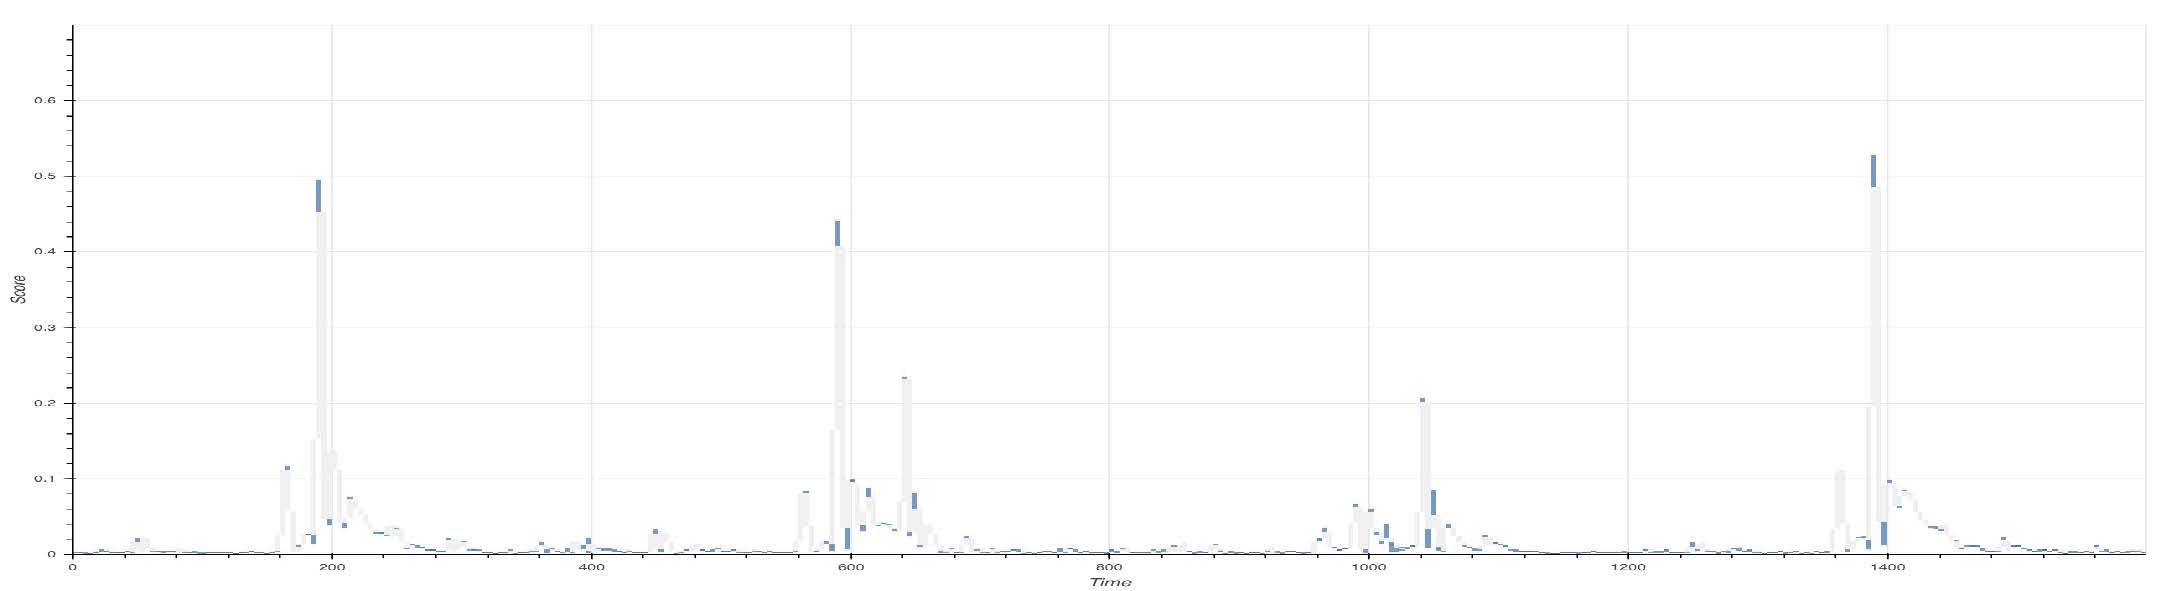
\includegraphics[width=\textwidth]{titansnr0123}
			\caption{$\tilde \nonce_i\in\{0,1,2,3\}$}
			\label{fig:titansnr0123}
		\end{subfigure}%
		\\% line break
		\begin{subfigure}[b]{\textwidth}
			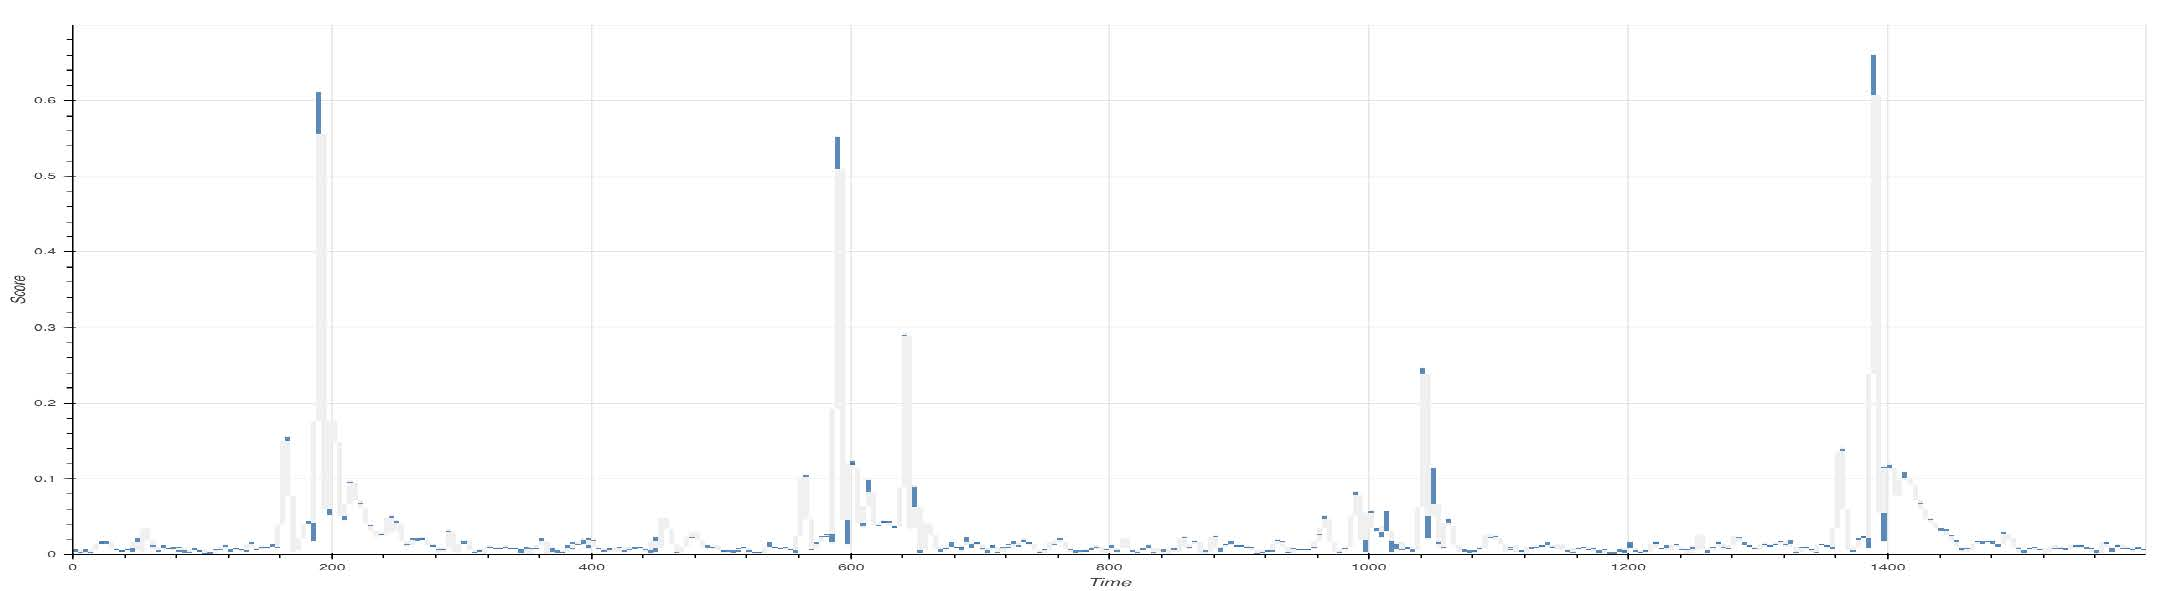
\includegraphics[width=\textwidth]{titansnr123}
			\caption{$\tilde \nonce_i\in\{1,2,3\}$}
			\label{fig:titansnr123}
		\end{subfigure}
		\bicaption{\enspace 信噪比结果}{\enspace SNR Results}
		\label{fig:titansnr}
	\end{figure}
	
	\algorithmref{alg:signscalar}只考虑了时间泄漏的防护。即使智能卡签名操作的数乘实现与\algorithmref{alg:signscalar}一致,也存在敏感数据泄漏的情况。Roche等\citep{Roche21}以\algorithmref{alg:signscalar}中的$\tilde \nonce_i$作为敏感中间值,对对齐后的电磁迹进行信噪比分析,实验结果如\figureref{fig:titansnr0123}所示。四类敏感中间值所计算出的SNR最大值为0.53。
	
	在\algorithmref{alg:signscalar}中$\tilde \multiplier_i\equiv \tilde\nonce_i$,当$\tilde \nonce_i=0$,虚拟的点加法$S+G_{\leakedmultiplier_i}$的被加数和加数实际上可以是任意两个椭圆曲线$E$上的点。Roche等\citep{Roche21}排除了敏感中间值$\tilde \nonce_i=0$时的能量迹重新计算SNR,实验结果如\figureref{fig:titansnr123}所示。三类敏感中间值所计算出的SNR最大值为0.65,相对于之前的信噪比有所提高,这说明对于$\tilde \nonce_i=0$这一类的点加法的电磁迹噪声较大,\algorithmref{alg:signscalar}第8行$\leakedmultiplier_i:=\tilde \nonce_i$很可能是错误的。
	
	Roche等\citep{Roche21}通过聚类的方法,验证了这样的事实:$\tilde \nonce_i=0$时,有$\frac12$的概率执行$\leakedmultiplier_i:=1$,有$\frac14$的概率执行$\leakedmultiplier_i:=2$,有$\frac14$的概率执行$\leakedmultiplier_i:=3$。Roche等\citep{Roche21}据此提出了更接近真实情况的签名操作的数乘实现的猜想,如\algorithmref{alg:improvesignscalar}所示。其中$G_1=G,G_2=2^{129}\cdot G,G_3=\left(2^{129}+1 \right) \cdot G,G_4=2^{128}\cdot G$。
	
	\begin{algorithm}
		\caption{改进后签名操作的数乘算法}\label{alg:improvesignscalar}
		\begin{algorithmic}[1]
			\Statex \textbf{输入:} $\left\{\tilde{\nonce}_0,\tilde{\nonce}_1,\dots,\tilde{\nonce}_i,\dots, \tilde{\nonce}_{128}\right\}$:一次性随机数$\nonce$的长度为129的编码形式
			\Statex \textbf{输入:} $G_1,G_2,G_3,G_4$:预计算的椭圆曲线$E$上的点
			\Statex \textbf{输出:} $\nonce\cdot G$:基点$G$与一次性随机数$\nonce$数乘的结果
			\State $S:=G_1$
			\For{$i=1,\dots , 128$}
			\State $S:=2\cdot S$
			\If {$\tilde \nonce_i>0$}
			\State $\leakedmultiplier_i:=\tilde \nonce_i$
			\State $S:=S+G_{\leakedmultiplier_i}$\Comment{$\leakedmultiplier_i$存在泄漏}
			\Else
			\State $\leakedmultiplier_i\stackrel{\$}\gets\{1,1,2,3\}$\Comment{引入随机数}
			\State $Dummy:=S+G_{\leakedmultiplier_i}$\Comment{$\leakedmultiplier_i$存在泄漏}
			\EndIf
			\EndFor
			\If {$\tilde \nonce_0=0$}
			\State $S:=S-G_4$
			\Else
			\State $Dummy:=S-G_4$
			\EndIf
			\State \Return $S$
		\end{algorithmic}
	\end{algorithm}
	
	\subsection{随机数部分泄漏的请况下基于格的对ECDSA的攻击}\label{subs:infoforlattice}
	
	有大量工作\citep{Howgrave-Graham01,Nguyen02,Nguyen03,Hlavac06,Brumley11,Mulder14,Benger14,Goudarzi16,Fan16,Ryan19,Jancar20,Moghimi20,Weiser20,Micheli20}研究了在随机数泄漏少量比特的情况下攻击ECDSA方案,它们的主要思想是利用签名中的随机数的泄漏构造扩展隐藏数问题\citep{Boneh96}的方程并使用格基规约求解。
	
	利用一次性随机数$\nonce$的泄漏求解私钥$\sk$不在本文研究范围内,因此只做大致描述。它求解私钥的流程如\figureref{fig:solver}所示,我们将利用随机数部分泄漏使用基于格的ECDSA攻击抽象为调用一个求解算法,使用$\mathcal S$表示求解算法。
	
	\begin{figure}[!htb]
		\centering
		\begin{tikzpicture}[node distance=20pt]
			\node[draw, rounded corners,align=center]  (start)  {运算开始};
			\node[draw, trapezium, trapezium left angle=70, trapezium right angle=110,below=of start,align=center](inputleak){输入:用于构造方程的签名及其泄漏};
			\node[draw, below=of inputleak,align=center] (constructequ)  {构造方程};
			\node[draw, below=of constructequ,align=center] (solve)  {使用格基规约算法求解};
			\node[draw, below=of solve,align=center] (calcd)  {根据最短向量求解私钥$\hat \sk$};
			\node[draw, diamond, aspect=2, below=of calcd,align=center]     (chkd)  {$\hat \sk\cdot G=\pk$?};
			
			\node[draw, trapezium, trapezium left angle=70, trapezium right angle=110,align=center]at ([xshift=-40pt,yshift=-35pt]chkd.south west)(success){输出:"求解成功",$\sk=\hat \sk$};
			\node[draw, trapezium, trapezium left angle=70, trapezium right angle=110,align=center]at ([xshift=40pt,yshift=-35pt]chkd.south east)(fail){输出:"求解失败"};
			\node[draw, rounded corners, below=50pt of chkd,align=center]  (end) {运算结束};
			
			\draw[->] (chkd) -|node[midway,very near start,above] {是} (success);
			\draw[->] (chkd) -|node[midway,very near start,above] {否} (fail);
			
			\draw[->] (success) |- (end);
			\draw[->] (fail) |- (end);
			\graph{
				(start)->(inputleak)->(constructequ)->(solve)->(calcd) -> (chkd);
			};
		\end{tikzpicture}
		\bicaption{\enspace 利用随机数部分泄漏使用基于格的ECDSA攻击流程图}{\enspace Flowchart of Lattice-based ECDSA Attacks with Partial Knowledge of the Nonces}
		\label{fig:solver}	
	\end{figure}
	
	$\mathcal S$是多项式时间复杂度的近似算法。只有构造方程签名中的的随机数泄漏需要同时满足三个限制时,$\mathcal S$才有较大可能在可接受的时间内求解出实际私钥$\sk$。三个限制如下所示。
	
	\begin{enumerate}
		\item 用于构造方程的签名中的随机数泄漏需要可利用;
		\item 用于构造方程的签名中的随机数泄漏需要足够多;
		\item 用于构造方程的签名中的随机数泄漏的准确率是100\%。
	\end{enumerate}
	
	本研究所使用的求解算法$\mathcal S$记为$S$。$S$求解时间约为400s。
	
	对于$S$,“可利用”指的是,恢复了\textbf{至少4个连续比特}签名中的一次性随机数$\nonce$泄漏以保证求解速度。如果使用没有4个连续比特随机数泄漏的签名构造方程,泄漏利用难度会增大,为了保证求解的正确性需要使用相对更多的签名,这会增加方程的维度从而增加求解时间。
	
	对于$S$,“足够多”指的是,需要\textbf{总共300比特}随机数泄漏的签名以构造正定或超定的方程,即需要$300\div 4=75$条有“可利用”随机数泄漏的签名。如果没有足够多的签名,那么构造的方程会欠定,这使得解空间变得非常大,无法求解实际私钥$d$。
	
	$S$对泄漏的准确率也有严格要求。这是因为一旦构造方程的泄漏存在错误(侧信道攻击恢复的数据与实际数据不一致),那么方程会错误,求解出的私钥与实际私钥$\sk$一定不符。
	\section{本章小结}
}
%"C:/Users/Administrator/Desktop/_毕业论文/context/附件4 中国科学院大学学位论文LaTeX模板2023.7.20/artratex.bat"